% fig_shell_crosssection.tex - Detailed cross-section of shell wall
% Standalone compilation: pdflatex fig_shell_crosssection.tex
\documentclass[tikz,border=5pt]{standalone}
\usepackage{tikz}
\usepackage{amsmath}
\usetikzlibrary{decorations.markings,arrows.meta,patterns,calc}

\begin{document}
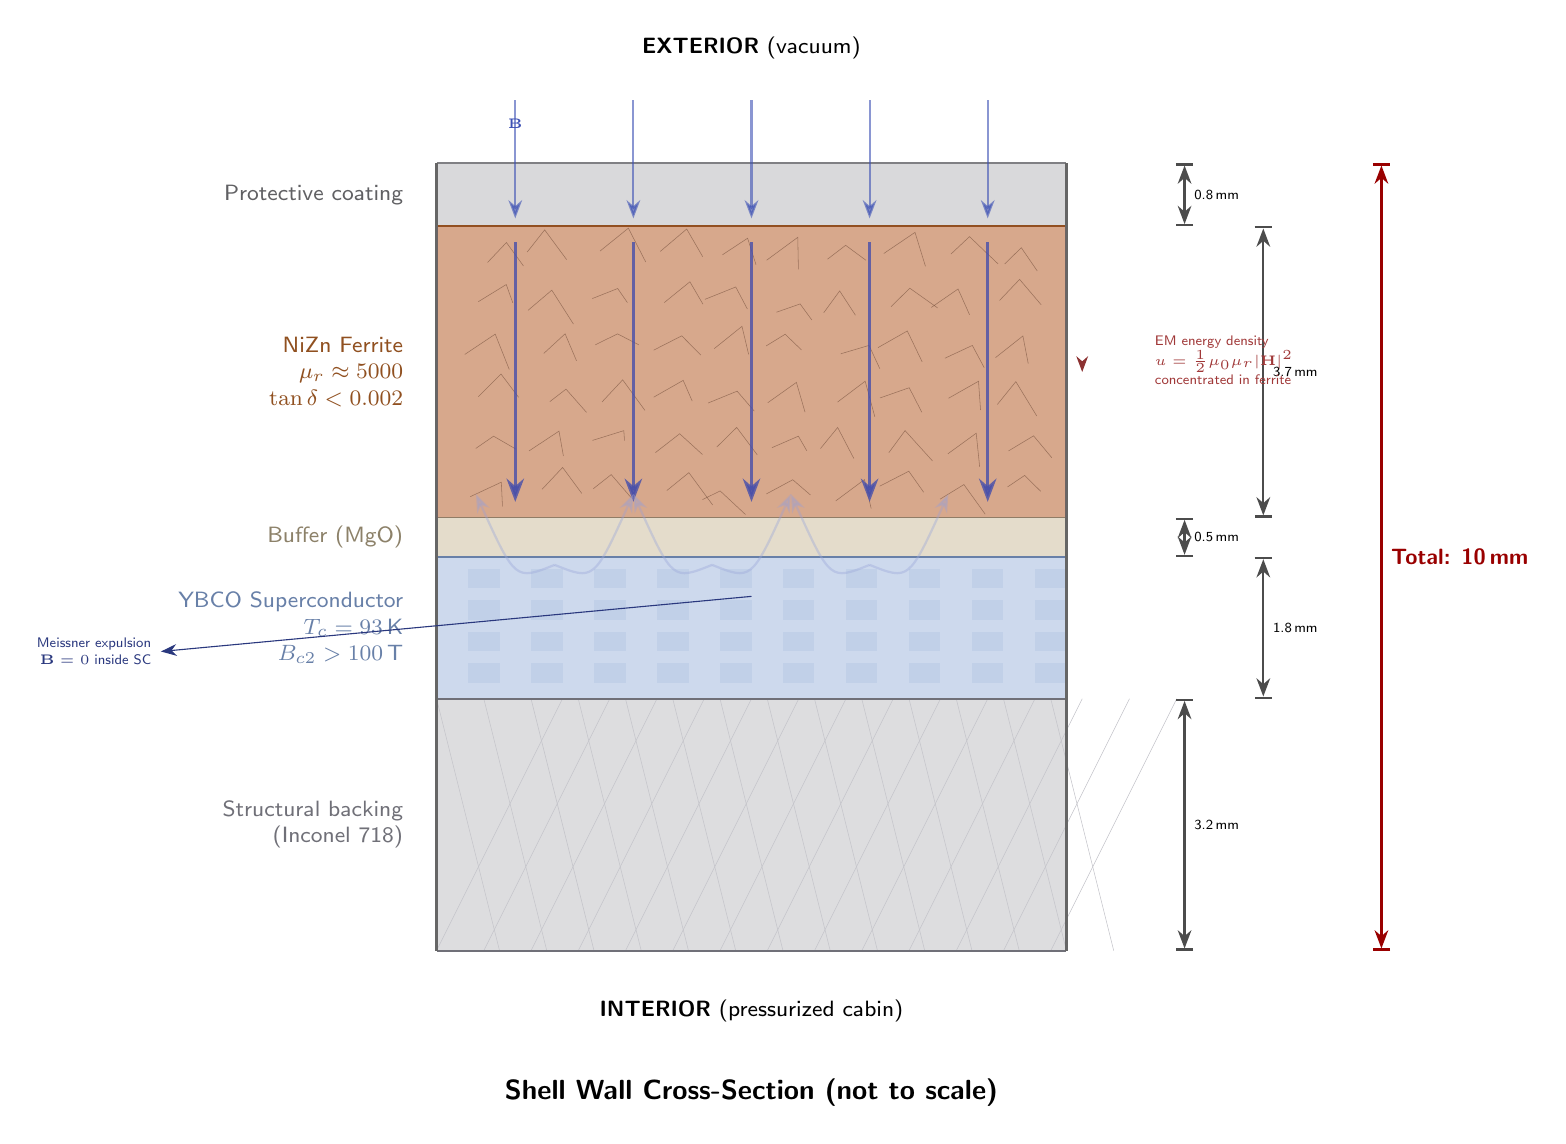
\begin{tikzpicture}[
    >=Stealth,
    every node/.style={font=\footnotesize\sffamily},
    dim/.style={|<->|, thick, black!70},
    matcallout/.style={draw=black!50, thin, -{Stealth[length=2mm]}},
]

% --- Define colors ---
\definecolor{coatingGray}{RGB}{160,160,165}
\definecolor{ferriteOrange}{RGB}{180,100,40}
\definecolor{ferriteLight}{RGB}{200,130,60}
\definecolor{bufferTan}{RGB}{200,185,150}
\definecolor{ybcoBlue}{RGB}{130,160,210}
\definecolor{ybcoLight}{RGB}{170,195,230}
\definecolor{structGray}{RGB}{140,140,150}
\definecolor{structLight}{RGB}{180,180,190}
\definecolor{emRed}{RGB}{200,70,70}
\definecolor{bfieldBlue}{RGB}{60,80,180}

% Layer thicknesses (scaled: 1 unit = ~1 mm in drawing)
\def\coatTop{10}    % Protective coating top
\def\coatBot{9.2}
\def\ferrTop{9.2}   % Ferrite layer top
\def\ferrBot{5.5}
\def\buffTop{5.5}   % Buffer layer top
\def\buffBot{5.0}
\def\ybcoTop{5.0}   % YBCO superconductor top
\def\ybcoBot{3.2}
\def\strTop{3.2}    % Structural backing top
\def\strBot{0}

\def\xL{0}          % Left edge
\def\xR{8}          % Right edge

% ============================================================
% LAYERS
% ============================================================

% --- Protective coating ---
\fill[coatingGray!40] (\xL,\coatBot) rectangle (\xR,\coatTop);
\draw[coatingGray!80!black, thick] (\xL,\coatTop) -- (\xR,\coatTop);
\draw[coatingGray!60!black] (\xL,\coatBot) -- (\xR,\coatBot);

% --- Ferrite layer (with grain structure) ---
\fill[ferriteOrange!50] (\xL,\ferrBot) rectangle (\xR,\ferrTop);
% Grain boundaries
\foreach \x in {0.5,1.3,2.0,2.8,3.5,4.2,5.0,5.7,6.4,7.2} {
    \foreach \y in {5.8,6.4,7.0,7.6,8.2,8.8} {
        \pgfmathsetmacro{\dx}{0.15*rand}
        \pgfmathsetmacro{\dy}{0.1*rand}
        \draw[ferriteOrange!30!black, very thin, opacity=0.4]
            ({\x+\dx},{\y+\dy}) -- +({0.3+0.1*rand},{0.2+0.1*rand})
            -- +({0.5+0.1*rand},{-0.1+0.1*rand});
    }
}
\draw[ferriteOrange!80!black, thick] (\xL,\ferrTop) -- (\xR,\ferrTop);
\draw[ferriteOrange!60!black] (\xL,\ferrBot) -- (\xR,\ferrBot);

% --- Buffer layer ---
\fill[bufferTan!50] (\xL,\buffBot) rectangle (\xR,\buffTop);
\draw[bufferTan!70!black] (\xL,\buffTop) -- (\xR,\buffTop);
\draw[bufferTan!70!black] (\xL,\buffBot) -- (\xR,\buffBot);

% --- YBCO superconductor ---
\fill[ybcoBlue!40] (\xL,\ybcoBot) rectangle (\xR,\ybcoTop);
% Crystal structure indication
\foreach \x in {0.4,1.2,2.0,2.8,3.6,4.4,5.2,6.0,6.8,7.6} {
    \foreach \y in {3.4,3.8,4.2,4.6} {
        \fill[ybcoBlue!70, opacity=0.3] (\x,\y) rectangle ++(0.4,0.25);
    }
}
\draw[ybcoBlue!80!black, thick] (\xL,\ybcoTop) -- (\xR,\ybcoTop);
\draw[ybcoBlue!70!black] (\xL,\ybcoBot) -- (\xR,\ybcoBot);

% --- Structural backing ---
\fill[structGray!30] (\xL,\strBot) rectangle (\xR,\strTop);
% Cross-hatching for structure
\foreach \x in {0,0.6,...,8} {
    \draw[structGray!50, very thin] (\x,\strBot) -- ({\x+1.6},\strTop);
    \draw[structGray!50, very thin] ({\x+0.8},\strBot) -- (\x,\strTop);
}
\draw[structGray!80!black, thick] (\xL,\strTop) -- (\xR,\strTop);
\draw[structGray!80!black, thick] (\xL,\strBot) -- (\xR,\strBot);

% --- Side borders ---
\draw[black!60, thick] (\xL,\strBot) -- (\xL,\coatTop);
\draw[black!60, thick] (\xR,\strBot) -- (\xR,\coatTop);

% ============================================================
% DIMENSION LINES (right side)
% ============================================================
\def\dimX{9.5}

% Coating
\draw[dim] (\dimX,\coatBot) -- (\dimX,\coatTop);
\node[right, font=\tiny\sffamily] at (\dimX,{(\coatTop+\coatBot)/2}) {0.8\,mm};

% Ferrite
\draw[dim] ({\dimX+1},\ferrBot) -- ({\dimX+1},\ferrTop);
\node[right, font=\tiny\sffamily] at ({\dimX+1},{(\ferrTop+\ferrBot)/2}) {3.7\,mm};

% Buffer
\draw[dim] (\dimX,\buffBot) -- (\dimX,\buffTop);
\node[right, font=\tiny\sffamily] at (\dimX,{(\buffTop+\buffBot)/2}) {0.5\,mm};

% YBCO
\draw[dim] ({\dimX+1},\ybcoBot) -- ({\dimX+1},\ybcoTop);
\node[right, font=\tiny\sffamily] at ({\dimX+1},{(\ybcoTop+\ybcoBot)/2}) {1.8\,mm};

% Structural
\draw[dim] (\dimX,\strBot) -- (\dimX,\strTop);
\node[right, font=\tiny\sffamily] at (\dimX,{(\strTop+\strBot)/2}) {3.2\,mm};

% Total
\draw[dim, red!60!black] ({\dimX+2.5},\strBot) -- ({\dimX+2.5},\coatTop);
\node[right, font=\footnotesize\sffamily\bfseries, red!60!black] at ({\dimX+2.5},5) {Total: 10\,mm};

% ============================================================
% LAYER LABELS (left side)
% ============================================================
\def\labX{-0.3}

\node[left, coatingGray!60!black] at (\labX,{(\coatTop+\coatBot)/2})
    {Protective coating};

\node[left, ferriteOrange!80!black, align=right] at (\labX,{(\ferrTop+\ferrBot)/2})
    {NiZn Ferrite\\$\mu_r \approx 5000$\\$\tan\delta < 0.002$};

\node[left, bufferTan!70!black] at (\labX,{(\buffTop+\buffBot)/2})
    {Buffer (MgO)};

\node[left, ybcoBlue!80!black, align=right] at (\labX,{(\ybcoTop+\ybcoBot)/2})
    {YBCO Superconductor\\$T_c = 93$\,K\\$B_{c2} > 100$\,T};

\node[left, structGray!80!black, align=right] at (\labX,{(\strTop+\strBot)/2})
    {Structural backing\\(Inconel 718)};

% ============================================================
% MAGNETIC FIELD PENETRATION (Meissner effect)
% ============================================================

% B-field arrows entering from top
\foreach \x in {1,2.5,4,5.5,7} {
    \draw[->, bfieldBlue, thick, opacity=0.6]
        (\x,\coatTop+0.8) -- (\x,\ferrTop+0.1);
}

% B-field concentrated in ferrite
\foreach \x in {1,2.5,4,5.5,7} {
    \draw[->, bfieldBlue, very thick, opacity=0.8]
        (\x,\ferrTop-0.2) -- (\x,\ferrBot+0.2);
}

% B-field expelled at superconductor (Meissner)
\foreach \x in {1.5,3.5,5.5} {
    \draw[->, bfieldBlue!50, thick, opacity=0.4]
        (\x,\buffBot-0.1) .. controls ({\x-0.5},\ybcoTop-0.3) .. ({\x-1},\buffTop+0.3);
    \draw[->, bfieldBlue!50, thick, opacity=0.4]
        (\x,\buffBot-0.1) .. controls ({\x+0.5},\ybcoTop-0.3) .. ({\x+1},\buffTop+0.3);
}

% Meissner effect label
\draw[matcallout, bfieldBlue!70!black] (4,\ybcoTop-0.5) -- (-3.5,3.8);
\node[left, bfieldBlue!70!black, align=right, font=\tiny\sffamily] at (-3.5,3.8)
    {Meissner expulsion\\$\mathbf{B} = 0$ inside SC};

% ============================================================
% EM ENERGY CONCENTRATION
% ============================================================

% Energy density shading in ferrite
\fill[emRed, opacity=0.08] (\xL,\ferrBot) rectangle (\xR,\ferrTop);

% Energy concentration arrows
\node[right, emRed!80!black, font=\tiny\sffamily, align=left] at (9,7.5)
    {EM energy density\\$u = \frac{1}{2}\mu_0\mu_r|\mathbf{H}|^2$\\concentrated in ferrite};
\draw[matcallout, emRed!70!black] (8.2,7.4) -- (8.2,{(\ferrTop+\ferrBot)/2});

% ============================================================
% OUTSIDE / INSIDE LABELS
% ============================================================
\node[font=\footnotesize\sffamily, anchor=south] at (4,\coatTop+1.2)
    {\textbf{EXTERIOR} (vacuum)};
\node[font=\footnotesize\sffamily, anchor=north] at (4,\strBot-0.5)
    {\textbf{INTERIOR} (pressurized cabin)};

% B-field label
\node[bfieldBlue, font=\tiny\sffamily] at (1,\coatTop+0.5) {$\mathbf{B}$};

% ============================================================
% TITLE
% ============================================================
\node[font=\normalsize\sffamily\bfseries, anchor=north] at (4,-1.5)
    {Shell Wall Cross-Section (not to scale)};

\end{tikzpicture}
\end{document}
